
In this final chapter, we want to look at a few ideas that are based on our extrapolation framework that could further improve the extrapolation of ground-state energies using neural networks.

In a first idea, we want to look at another training modification which will work by dynamically filtering frequencies.

In a second idea, we demonstrate the effect of preselecting frequencies on the extrapolation.

Last, we want to outlay three different general approaches to the idea of using neural networks as an extrapolation tool for ground-state energies.
\section{Frequency filter}
\begin{wrapfigure}{r}{.5\textwidth}
  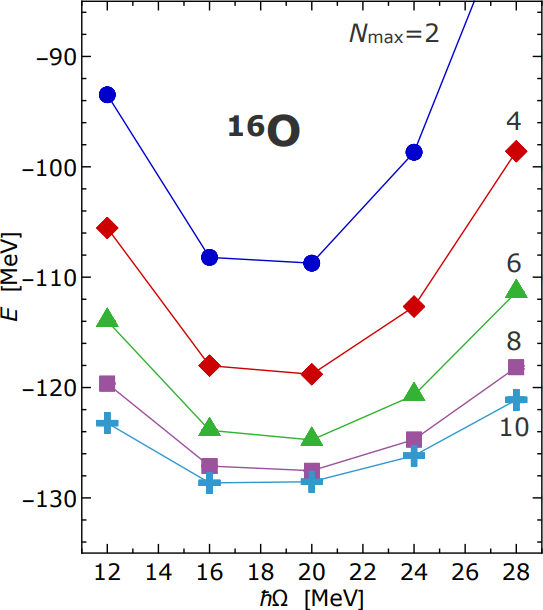
\includegraphics[width=.5\textwidth]{media/freq_filter.png}
  \caption{NCSM calculations for \n{16}{O} in dependency on the used oscillator frequency \cite{sommerschule}.}
  \label{fig:freq_dependency}
\end{wrapfigure}
The single-particle harmonic oscillator basis is not asymptotically good to approximate the states of nuclei, as harmonic oscillator wave functions fall off like a gaussian function, but bound states in a potential well typically fall off like an exponential function \cite{sommerschule}. Furthermore, the composition into the harmonic oscillator Slater determinants is dependant on a free parameter for the oscillator frequency. This oscillator frequency also defines the oscillator length and thus the spatial resolution for the basis states.

As we have already seen, the dependence on the oscillator frequency results in different convergence rates for our NCSM sequences. In fact, NCSM calculations using harmonic oscillator Slater determinants typically show a parabolic convergence behaviour with respect to the used oscillator frequency. This is shown in \autoref{fig:freq_dependency} for the nucleus \n{16}{O}. As a consequence, there is a special frequency, for which an optimal convergence rate is to be expected. In \autoref{fig:freq_dependency}, this minimum frequency is given by $\hbar \Omega = \SI{20}{\mega\electronvolt}$.

In order to capture those different convergence rates, we want to restrict the sequences used to either side of the minimum, resulting in two training modes. In the first training mode, only sequences smaller than the frequency minimum are used, such that the network will get more information of the long range behaviour of the nucleonic interaction. As a result, the networks have to model the short range behaviour. Conversely, in the second training mode, the networks will be trained on the short range behaviour by restricting the frequencies to the ones higher than the minimum, thus modeling long range behaviour.

To implement this, we dynamically compute the frequency, for which the lowest value is achieved at $N_\mathrm{max} = 8$ for each NCSM calculation. This frequency will be used to filter the frequencies for the training. In both cases, we include the frequency minimum, as that is the frequency with the best convergence behaviour.



\begin{figure}[H]
  \begin{subfigure}{\textwidth}
    \centering
    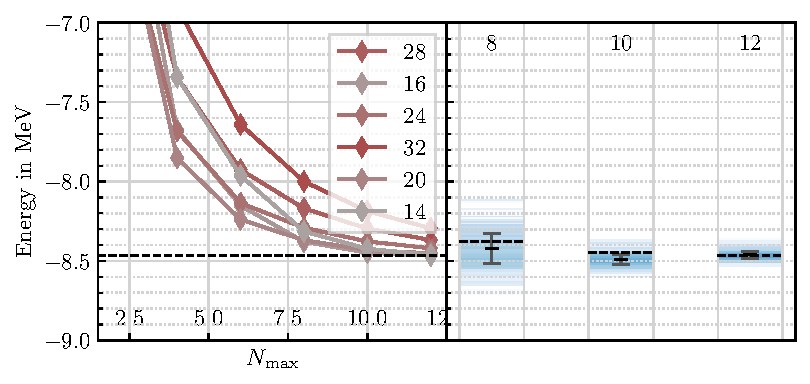
\includegraphics{media/outlook_frequency_lower.pdf}
    \caption{}
  \end{subfigure}
  \begin{subfigure}{\textwidth}
    \centering
    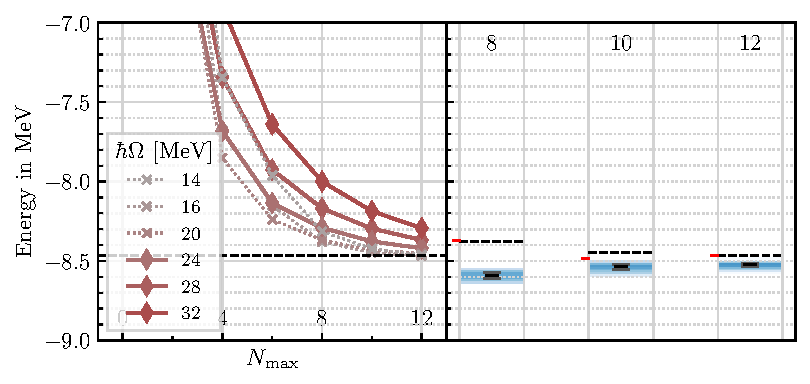
\includegraphics{media/outlook_frequency_higher.pdf}
    \caption{}
  \end{subfigure}
  \caption{Evaluation of the frequency filter training mode on \n{3}{H} with the interaction specified above. The frequencies used in the evaluation are shown with solid lines. To achieve a better comparability with the previous extrapolations, the frequencies not taken into account are shown as dotted lines. In \textbf{(a)}, the networks were trained on the low frequencies, thus modeling the short range behaviour. In \textbf{(b)}, the networks were trained on the high frequencies, thus modeling the long range behaviour.}
  \label{fig:eval_freqfilter}
\end{figure}

We look at a single example of the \n{3}{H} nucleus, using a semi-local momentum space regulated N$^{4}$LO interaction with two-body interactions and a cutoff at \SI{450}{\mega\electronvolt} alongside a SRG evolution with a flow parameter of \srg{0.08}. Since there are six frequencies available, the evaluation for the long range training mode will include the three lowest and the evaluation for the short range mode will include the three highest frequencies. In \autoref{fig:eval_freqfilter}, the evaluation results are seen for the difference-based extrapolation framework.

In the case where the networks have been trained on the low frequencies, the prediction for $N_\mathrm{max} = 8$ is too high. Also, the uncertainty is still very large, which stabilizes along with the value of the predictions for $N_\mathrm{max} \geq 10$, where the range of the predictions get much smaller. If we look at the evaluation data at $N_\mathrm{max} = 8$, we see that the sequence for $\hbar\Omega = \SI{14}{\mega\electronvolt}$ is still very steep compared to the other two sequences. As we have already seen, this broad range between different slopes result in a larger range of predictions. At $N_\mathrm{max} = 10$ the sequences converge much more uniformly, leading to the more precise predictions.

In contrast to the training with lower frequencies, the behaviour predictions of the training with higher frequencies look more consistent across the different $N_\mathrm{max}$. For every $N_\mathrm{max}$, the networks predict ground-state energies which are too low, but correct those to higher values with rising $N_\mathrm{max}$, similar to the observations made in the absolute-based framework. Here, the sequences of the higher frequencies converge much more uniformly, which is the reason we cannot confidentially attribute the precision of the networks prediction to the fact of them being only trained on the high frequencies. To further analyze the behaviour of the networks when trained only on short or long ranges, more investigations need to be done on nuclei which show different ranges of slopes for the high and for the low frequencies.

\section{Frequency selection}
In both of our extrapolation frameworks, we deliberately considered every available frequency to predict the ground-state energy, since we wanted to obtain a more general extrapolation. This "black-box" behaviour could lead to worse predictions, but does not require a hand-selection of a subset of the sequences for extrapolation. Also, this would require a metric on what sequences to choose. For ground-state energies, the convergence is monotonic and decreasing, such that we \textit{could} choose such a metric, where we choose the three sequences, for which the value at the highest $N_\mathrm{max}$ are the lowest among all sequences available. We want to demonstrate this frequency preselection idea by evaluating the \n{2}{H} nucleus using the same interaction as in the previous chapters with a flow parameter of \srg{0.08}.

In \autoref{fig:eval_freqselection}, the results are shown. If we compare these results to the results of the unmodified training in \autoref{fig:eval_diff} for the \srg{0.08} interaction of \n{2}{H}, we can see that the frequency preselection significantly improves the absolute value, as well as the uncertainty of the prediction for the $N_\mathrm{max}$ values of $8$ and $10$.

Of course, manually selecting the sequences which will be used in evaluation with a predefined metric limits the extrapolation framework to the types of observables for which this metric can apply. For example, after we have decided to only use the sequences with the three lowest values at the highest $N_\mathrm{max}$, the framework gets limited to ground-state energies. The extrapolation of other observables, that do not show the monotone decreasing convergence behaviour of the ground-state energy will therefore not be optimized.

In the end, the decision to use a manual preselection of frequency is a tradeoff between a framework with more precise and more accurate predictions and a framework which is more general.

If one decides to manually preselect frequencies for evaluation, it may be of interest to also develop and analyze different metrics for choosing such sequences. In the case of our ground-state energy extrapolation framework, we chose the lowest sequences as the best sequences to choose. Another possibility would be to choose the three sequences which show the most uniform convergence behaviour, as we have observed that this significantly lowers the uncertainty in the predictions.

\begin{figure}[H]
  \centering
  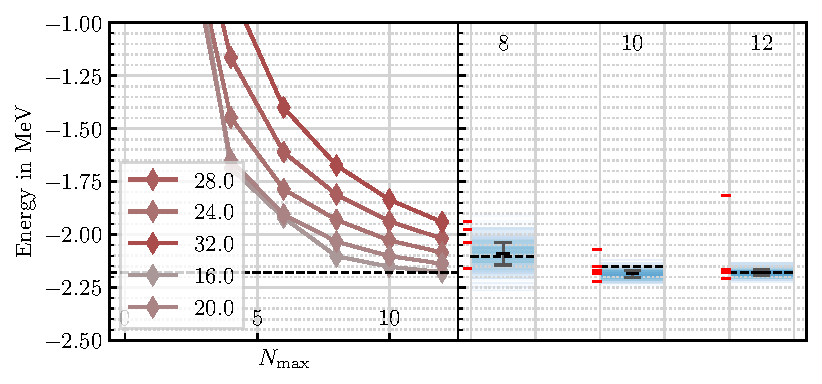
\includegraphics{media/outlook_selection.pdf}
  \caption{Evaluation of the \n{2}{H} nucleus in the difference based framework using only the three lowest frequencies. In this case, the frequencies are $\hbar\Omega = 16, 20, \SI{24}{\mega\electronvolt}$. The frequencies used in the evaluation are shown with solid lines. To achieve a better comparability to the previous extrapolations, the frequencies not taken into account are shown as dotted lines.}
  \label{fig:eval_freqselection}
\end{figure}

\section{Norming and monotonicity}
\input{chapters/8_outlook/further.tex}
